20. $\cfrac{(x-1)(x-2)}{x^2+7x+12}\leqslant1\Leftrightarrow \cfrac{x^2-2x-x+2-x^2-7x-12}{x^2+7x+12}\leqslant0
\Leftrightarrow \cfrac{-10(x+1)}{(x+3)(x+4)}\leqslant0.$ Применив метод интервалов, найдём ответ: $x\in(-4;-3)\cup[-1;+\infty).$
\begin{figure}[ht!]
\center{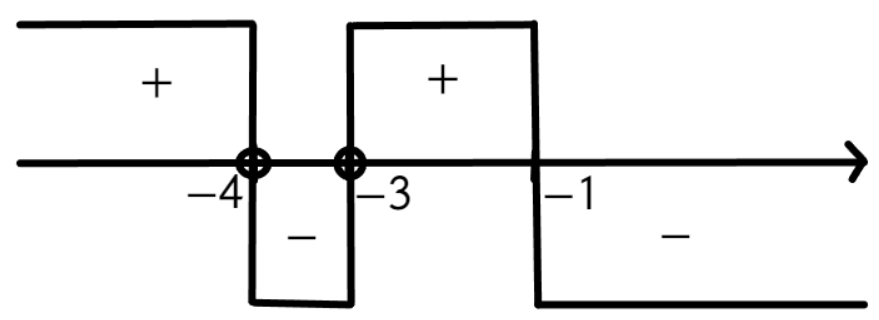
\includegraphics[scale=0.35]{ner9-20.png}}
\end{figure}\\
